\documentclass[a4paper,11pt]{ltjsarticle}
\usepackage[dvipdfmx]{graphicx}
\usepackage{color}
\usepackage{amssymb}
\usepackage{here}
\usepackage{subcaption}
\usepackage{amsmath}
\usepackage{listings}
\usepackage{url}

\lstset{
	%プログラム言語(複数の言語に対応,C,C++も可)
	language = Matlab,
	%背景色と透過度
	backgroundcolor={\color[gray]{.90}},
	%枠外に行った時の自動改行
	breaklines = true,
	%自動改行後のインデント量(デフォルトでは20[pt])	
	breakindent = 10pt,
	%標準の書体
	basicstyle = \ttfamily\scriptsize,
	%コメントの書体
	commentstyle = {\itshape \color[cmyk]{1,0.4,1,0}},
	%関数名等の色の設定
	classoffset = 0,
	%キーワード(int, ifなど)の書体
	keywordstyle = {\bfseries \color[cmyk]{0,1,0,0}},
	%表示する文字の書体
	stringstyle = {\ttfamily \color[rgb]{0,0,1}},
	%枠 "t"は上に線を記載, "T"は上に二重線を記載
 %他オプション:leftline,topline,bottomline,lines,single,shadowbox
	frame = TBrl,
	%frameまでの間隔(行番号とプログラムの間)
	framesep = 5pt,
	%行番号の位置
	numbers = left,
 %行番号の間隔
	stepnumber = 1,
 %行番号の書体
	numberstyle = \tiny,
 %タブの大きさ
	tabsize = 4,
	%キャプションの場所("tb"ならば上下両方に記載)
	captionpos = t
}
\begin{document}

\title{信号処理 課題レポート(2)}
\author{学籍番号:2022531033 氏名:関川謙人}
\date{提出日:\today}
\maketitle

\section*{課題1}
次の語句について知っていることを簡潔に述べよ
\subsection*{(1)シャノンのサンプリング定理}
アナログ信号をディジタル信号にサンプリングする際に重要な定理で
音声処理や画像処理などに利用される。
\subsection*{(2)短時間フーリエ変換}
長い信号を逐次的に解析する場合に利用する、信号を適度な長さに切りだした後、
窓関数をかけてフーリエ変換(解析)を行う手法。
\subsection*{課題2}
\subsubsection*{(1)逆離散フーリエ変換プログラム}
逆離散フーリエ変換を実行及び検証するプログラムを以下に示す。
\lstinputlisting[title={myidft2024.m}]{DSP1/myidft2024.m}

\subsection*{(2)}
%横に3枚の画像(jpg/png)表示
\begin{figure}[H]
\begin{center}
\begin{tabular}{c}
\begin{minipage}{0.33\hsize}
\begin{center}
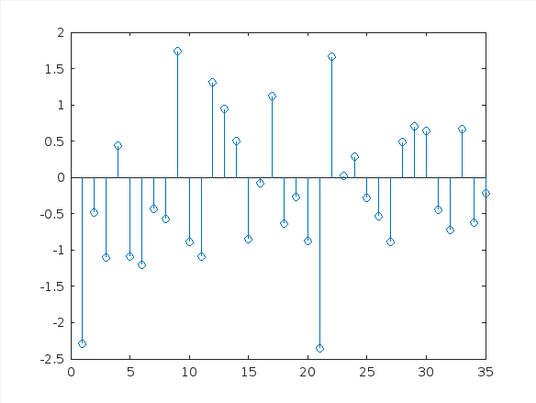
\includegraphics[width=5cm]{DSP1/R2_2_1.png}
\end{center}
\caption{変換前の信号}
\label{image1}
\end{minipage}
\begin{minipage}{0.33\hsize}
\begin{center}
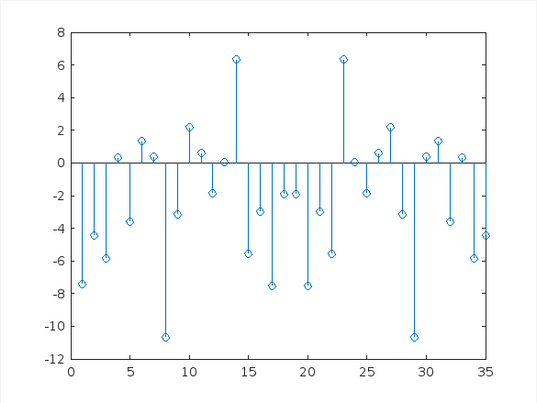
\includegraphics[width=5cm]{DSP1/R2_2_2.png}
\end{center}
\caption{変換後の信号}
\label{image2}
\end{minipage}
\begin{minipage}{0.33\hsize}
\begin{center}
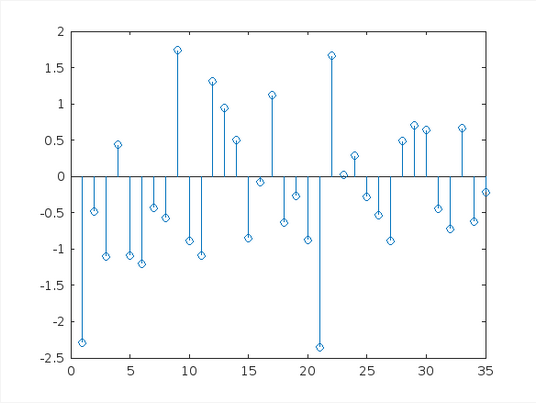
\includegraphics[width=5cm]{DSP1/R2_2_3.png}
\end{center}
\caption{逆変換でもとに戻した信号}
\label{image3}
\end{minipage}
\end{tabular}
\end{center}
\end{figure}

\ref{image1}と\ref{image3}がほぼ同じ形であるため、mydft2024で変換した
信号から、myidft2024.mにより元の信号が得られる。

\section*{課題3}
差分方程式が以下で与えられる線形時不変システムについて以下の問いに答えよ。
\begin{equation*}
	y(n) = -2x(n) + 4x(n-1) + 3ay(n-1) - 2a^{2}y(n-2)
\end{equation*}
\subsection*{(1)回路図を示せ}

以下に回路図を示す。
\begin{figure}[H]
\begin{center}
\includegraphics*[height = 8cm]{DSP1/R2_3_1.png}
\caption{回路図}
\end{center}
\end{figure}

\subsection*{(2)$n=0,1,2,3$におけるインパルス応答を求めよ}
インパルス応答において、基本的に入力$x(n)$はデルタ関数$\delta (n)$となる。

$n=0$の時、$x(0) = 1$であり、それ以外は0。
よって以下のようになる。
\begin{align*}
	y(0) &= -2x(0) + 4x(-1) + 3ay(-1) - 2a^{2}y(-2) \\
	&= -2
\end{align*}

$n = 1$の時、
\begin{align*}
	y(1) &= -2x(1) + 4x(0) + 3ay(0) - 2a^{2}y(-1) \\
	&= -6a + 4
\end{align*}

$n = 2$の時、
\begin{align*}
	y(2) &= -2x(2) + 4x(1) + 3ay(1) - 2a^{2}y(0) \\
	&= 3a(-6a + 4) - 2a^{2} \times -2 \\
	&= -14a^{2} + 12a
\end{align*}

$n = 3$の時
\begin{align*}
	y(3) &= -2x(3) + 4x(2) + 3ay(2) - 2a^{2}y(1) \\
	&= 3a(-14a^{2} + 12a) - 2a^{2}(-6a + 4) \\
	&= -42a^{3} + 36a^{2} + 12a^{3} - 8a^{2} \\
	&= -30a^{3} + 28a^{2}
\end{align*}

\subsection*{(3)伝達関数を求めよ}
$y(n)$をZ変換すると
\begin{equation*}
	Y(z)=-2X(z) + 4X(z)z^{-1} + 3aY(z)z^{-1} -2a^{2}Y(z)z^{-2}
\end{equation*}
となる。これYに関する項を左辺、Xに関する項を右辺に移動させると、
\begin{equation*}
	Y(z)[1 - 3az^{-1} + 2a^{2}z^{-2}] = 
	X(z)[-2 + 4z^{-1}]
\end{equation*}
よって、伝達関数$H(z)$は、
\begin{align*}
	H(z) &= \frac{Y(z)}{X(z)} \\
	&= \frac{-2 + 4z^{-1}}{1 - 3az^{-1} + 2a^{2}z^{-2}}
\end{align*}
となる。
\subsection*{(4)極を求めよ}
極は伝達関数の分母の根となる。分母である
${1 - 3az^{-1} + 2a^{2}z^{-2}} = 0$のzの値を求めることで
極を求めることができる。この式は$(z-a)(z-2a)$の形に分解できるため、
システムの極は$a,2a$とみることができる。

\section*{課題4}
周期0.002[sec]でサンプリングされた信号$x(n)$の振幅スペクト
ルが下図である

\subsection*{(1)この信号のサンプリング周波数はいくらか}
周期$T=0.002$[s]であるため、サンプリング周波数は、

$\frac{1}{T} = \frac{1}{0.002} = 500$[Hz]

よって500[Hz]となる。

\subsection*{(2)Aを求めよ。}
離散時間信号において、角周波数2πの時は、500[Hz]に相当する。
このことから、$\pi$は250[Hz]に相当すると考えられる。

\subsection*{(3)振幅スペクトルの概略図を$[-\pi,\pi]$の範囲で書け}
\begin{figure}[H]
\begin{center}
\includegraphics*[height = 8cm]{DSP1/R2_4_3.png}
\caption{}
\end{center}
\end{figure}

\subsection*{(4)この信号の特徴を周波数という言葉を用いて簡潔に述べよ。}
この信号は500[Hz]の周波数でサンプリングされている信号である。
また、最大周波数は250Hzである。また、この信号は、$a$などの特定の
周波数の時、スペクトルの振幅が大きくなる。

\subsection*{(5)$[b,\pi]$の区間のスペクトルだけ削除したい。どのような振幅特性を
持つフィルタをかければよいか。概略図を赤色で記せ。}
\begin{figure}[H]
\begin{center}
\includegraphics*[height = 8cm]{DSP1/R2_5_5.png}
\caption{}
\end{center}
\end{figure}

\end{document}